\chapter{The O'Briens in Ireland}

The family of William O'Brien and Mary Sexton came to America from the town of Watergrasshill in County Cork, Ireland.\citep{Edward2OBrienNaturalization,Michael2OBrienNaturalization,Margaret3DooleyBaptism} The village of Watergrasshill is situated mostly within the civil parish of Ardnageehy and partly within Kilquane, in the larger barony of Barrymore, on the main road between Cork and Dublin.\citep{TopographicalDictionary} The name Watergrasshill was originally ``Watercress Hill,'' and in Irish is \textit{Cnoc\'{a}n-na-biolraighe} (Knockaun-na-billery).\citep{LocalNames}

\begin{figure}
	\centering
	\includegraphics[width=\textwidth]{ireland_map}
	\caption{Map of Ireland with pin indicating the location of Watergrasshill}
\end{figure}

\begin{figure}
	\centering
	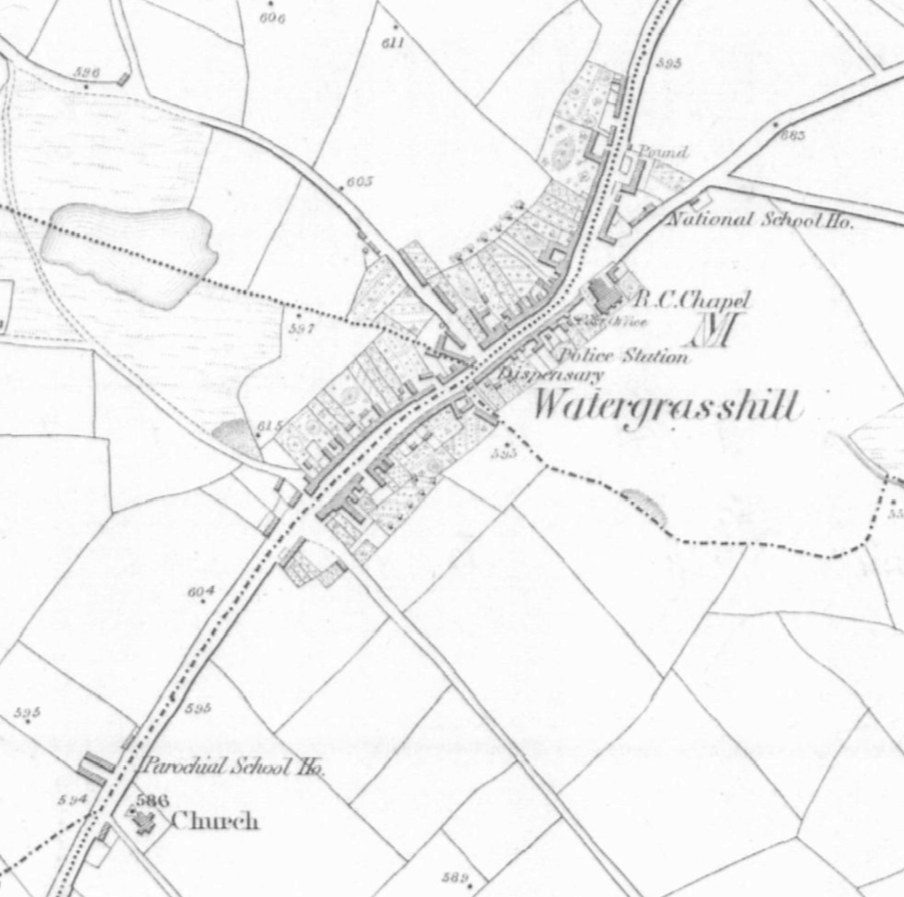
\includegraphics[width=\textwidth]{watergrasshill_cropped}
	\caption{Historic map of Watergrasshill, Ordnance Survey Ireland, map series ``Historic 6" First Edition B\&W (1829--41)'', scale 1:5,000, map sheet CK053}
\end{figure}

Watergrasshill was a small town of 801 inhabitants in 1841, when William and his family lived there prior to their emigration to the U.S. By 1871 the population had dropped to 143.\citep{Population} Some of this population loss was likely due to the famine, but the arrival of the railroad may also have played a role. The Great Southern and Western Railway reached the City of Cork in 1849.\citep{Bianconi} Two people performing land valuations included their impressions of Watergrasshill and its transformation. D.\ Quinn wrote in Feb 1849:

\begin{quote}
	This Town is Poor, but a great deal is done in the way of ``Carmen's Stages,'' it being on the Dublin line to Cork and half way (11 miles) from the latter City to Fermoy -- a good deal of benefit is done the Town by these persons ---\citep{HouseIntro}
\end{quote}

J.\ Montgomery wrote in Dec 1852 and sometime prior:

\begin{quote}
	2 coaches \& Bianconis\footnote{Charles Bianconi was an Italian entrepreneur who operated passenger coaches between cities throughout Ireland.\citep{Bianconi}} can pass through the village daily \& change Horses here -- one or two individuals are thus making pretty well by this -- by the rent for stabling \&c -- \& when the railway to Cork is finished, it will lose a good part of this advantage ---
	
	It has lost a great deal of it now -- (1852) but it is the best of the little villages in this neighborhood although poor enough -- Poor Rates are low -- only 1/7th for 1832 \& none at all in 1837 -- Those made a moderate val\textsuperscript{n}.\ considering these circumstances.\citep{HouseIntro}
\end{quote}

There are few Irish records available covering the early 19th century. Civil registration of births, marriages, and deaths didn't fully occur in Ireland until 1864.\citep{Grenham1} Census records prior to 1901 were mostly lost in a 1922 fire at the Public Records Office.\citep{Grenham18} However, there are O'Briens in Watergrasshill who appear in name directories and Griffith's Valuation records from the time period when William's family lived in the area. It's possible that these sources may reveal some small details about the family's life in Ireland. 

There is a ``W\textsuperscript{m}.\ Brien'' listed in the town of Watergrasshill who was leasing a house with a yard and garden.\cite{House1849:4} The Feb 1849 revision has William's name crossed out and the word ``Vact.''\ written, indicating that the house was vacant and William had moved away.\citep{House1849-2} There are no other William O'Briens or similar name variants listed in Watergrasshill, although other O'Briens in town include Denis,\cite{House1849:6dennis} Owen,\cite{House1849:6owen} Patrick,\cite{House1849:7} and Margaret.\cite{House1849:11}

The final version of Griffith's Valuation, published in 1853, shows only Owen O'Brien\cite{Griffiths:46,Griffiths:90} and Patrick O'Brien\cite{Griffiths:90} remaining in Watergrasshill.\footnote{There are two properties occupied by an Owen O'Brien and two properties occupied by a Patrick O'Brien. It's unknown whether these are four separate individuals or if there may be multiple properties rented by the same individuals.} By 1901 it appears that all O'Briens had left Watergrasshill, as none are listed in the 1901 or 1911 census.\cite{1901IrishCensus,1911IrishCensus}

The departure of the O'Brien family from Ireland corresponded with the ending years of the Irish potato famine, also known as the Great Famine, which lasted from 1845--1849. During this time, there were between 1.5 and 3 million famine-related deaths in Ireland and 1 million people left Ireland for North America.\cite{Smith:469}

Watergrasshill was a poor town in the 1840s that was largely sustained by horse travel between Dublin and Cork. With the loss of that business to the railway and the effects of the famine, it made sense for the O'Brien family to look for new opportunities in America.

